\documentclass[12pt]{article}

%packages
%\usepackage{latexsym}
\usepackage{graphicx}
\usepackage{color}
\usepackage{amsmath}
\usepackage{dsfont}
\usepackage{placeins}
\usepackage{amssymb}
\usepackage{wasysym}
\usepackage{abstract}
\usepackage{hyperref}
\usepackage{etoolbox}
\usepackage{datetime}
\usepackage{xcolor}
\usepackage{alphalph}
\settimeformat{ampmtime}

%\usepackage{pstricks,pst-node,pst-tree}

%\usepackage{algpseudocode}
%\usepackage{amsthm}
%\usepackage{hyperref}
%\usepackage{mathrsfs}
%\usepackage{amsfonts}
%\usepackage{bbding}
%\usepackage{listings}
%\usepackage{appendix}
\usepackage[margin=1in]{geometry}
%\geometry{papersize={8.5in,11in},total={6.5in,9in}}
%\usepackage{cancel}
%\usepackage{algorithmic, algorithm}

\makeatletter
\def\maxwidth{ %
  \ifdim\Gin@nat@width>\linewidth
    \linewidth
  \else
    \Gin@nat@width
  \fi
}
\makeatother

\definecolor{fgcolor}{rgb}{0.345, 0.345, 0.345}
\newcommand{\hlnum}[1]{\textcolor[rgb]{0.686,0.059,0.569}{#1}}%
\newcommand{\hlstr}[1]{\textcolor[rgb]{0.192,0.494,0.8}{#1}}%
\newcommand{\hlcom}[1]{\textcolor[rgb]{0.678,0.584,0.686}{\textit{#1}}}%
\newcommand{\hlopt}[1]{\textcolor[rgb]{0,0,0}{#1}}%
\newcommand{\hlstd}[1]{\textcolor[rgb]{0.345,0.345,0.345}{#1}}%
\newcommand{\hlkwa}[1]{\textcolor[rgb]{0.161,0.373,0.58}{\textbf{#1}}}%
\newcommand{\hlkwb}[1]{\textcolor[rgb]{0.69,0.353,0.396}{#1}}%
\newcommand{\hlkwc}[1]{\textcolor[rgb]{0.333,0.667,0.333}{#1}}%
\newcommand{\hlkwd}[1]{\textcolor[rgb]{0.737,0.353,0.396}{\textbf{#1}}}%

\usepackage{framed}
\makeatletter
\newenvironment{kframe}{%
 \def\at@end@of@kframe{}%
 \ifinner\ifhmode%
  \def\at@end@of@kframe{\end{minipage}}%
  \begin{minipage}{\columnwidth}%
 \fi\fi%
 \def\FrameCommand##1{\hskip\@totalleftmargin \hskip-\fboxsep
 \colorbox{shadecolor}{##1}\hskip-\fboxsep
     % There is no \\@totalrightmargin, so:
     \hskip-\linewidth \hskip-\@totalleftmargin \hskip\columnwidth}%
 \MakeFramed {\advance\hsize-\width
   \@totalleftmargin\z@ \linewidth\hsize
   \@setminipage}}%
 {\par\unskip\endMakeFramed%
 \at@end@of@kframe}
\makeatother

\definecolor{shadecolor}{rgb}{.77, .77, .77}
\definecolor{messagecolor}{rgb}{0, 0, 0}
\definecolor{warningcolor}{rgb}{1, 0, 1}
\definecolor{errorcolor}{rgb}{1, 0, 0}
\newenvironment{knitrout}{}{} % an empty environment to be redefined in TeX

\usepackage{alltt}
\usepackage[T1]{fontenc}

\newcommand{\qu}[1]{``#1''}
\newcounter{probnum}
\setcounter{probnum}{1}

%create definition to allow local margin changes
\def\changemargin#1#2{\list{}{\rightmargin#2\leftmargin#1}\item[]}
\let\endchangemargin=\endlist 

%allow equations to span multiple pages
\allowdisplaybreaks

%define colors and color typesetting conveniences
\definecolor{gray}{rgb}{0.5,0.5,0.5}
\definecolor{black}{rgb}{0,0,0}
\definecolor{white}{rgb}{1,1,1}
\definecolor{blue}{rgb}{0.5,0.5,1}
\newcommand{\inblue}[1]{\color{blue}#1 \color{black}}
\definecolor{green}{rgb}{0.133,0.545,0.133}
\newcommand{\ingreen}[1]{\color{green}#1 \color{black}}
\definecolor{yellow}{rgb}{1,1,0}
\newcommand{\inyellow}[1]{\color{yellow}#1 \color{black}}
\definecolor{orange}{rgb}{0.9,0.649,0}
\newcommand{\inorange}[1]{\color{orange}#1 \color{black}}
\definecolor{red}{rgb}{1,0.133,0.133}
\newcommand{\inred}[1]{\color{red}#1 \color{black}}
\definecolor{purple}{rgb}{0.58,0,0.827}
\newcommand{\inpurple}[1]{\color{purple}#1 \color{black}}
\definecolor{backgcode}{rgb}{0.97,0.97,0.8}
\definecolor{Brown}{cmyk}{0,0.81,1,0.60}
\definecolor{OliveGreen}{cmyk}{0.64,0,0.95,0.40}
\definecolor{CadetBlue}{cmyk}{0.62,0.57,0.23,0}

%define new math operators
\DeclareMathOperator*{\argmax}{arg\,max~}
\DeclareMathOperator*{\argmin}{arg\,min~}
\DeclareMathOperator*{\argsup}{arg\,sup~}
\DeclareMathOperator*{\arginf}{arg\,inf~}
\DeclareMathOperator*{\convolution}{\text{\Huge{$\ast$}}}
\newcommand{\infconv}[2]{\convolution^\infty_{#1 = 1} #2}
%true functions

%%%% GENERAL SHORTCUTS

%shortcuts for pure typesetting conveniences
\newcommand{\bv}[1]{\boldsymbol{#1}}

%shortcuts for compound constants
\newcommand{\BetaDistrConst}{\dfrac{\Gamma(\alpha + \beta)}{\Gamma(\alpha)\Gamma(\beta)}}
\newcommand{\NormDistrConst}{\dfrac{1}{\sqrt{2\pi\sigma^2}}}

%shortcuts for conventional symbols
\newcommand{\tsq}{\tau^2}
\newcommand{\tsqh}{\hat{\tau}^2}
\newcommand{\sigsq}{\sigma^2}
\newcommand{\sigsqsq}{\parens{\sigma^2}^2}
\newcommand{\sigsqovern}{\dfrac{\sigsq}{n}}
\newcommand{\tausq}{\tau^2}
\newcommand{\tausqalpha}{\tau^2_\alpha}
\newcommand{\tausqbeta}{\tau^2_\beta}
\newcommand{\tausqsigma}{\tau^2_\sigma}
\newcommand{\betasq}{\beta^2}
\newcommand{\sigsqvec}{\bv{\sigma}^2}
\newcommand{\sigsqhat}{\hat{\sigma}^2}
\newcommand{\sigsqhatmlebayes}{\sigsqhat_{\text{Bayes, MLE}}}
\newcommand{\sigsqhatmle}[1]{\sigsqhat_{#1, \text{MLE}}}
\newcommand{\bSigma}{\bv{\Sigma}}
\newcommand{\bSigmainv}{\bSigma^{-1}}
\newcommand{\thetavec}{\bv{\theta}}
\newcommand{\thetahat}{\hat{\theta}}
\newcommand{\thetahatmle}{\hat{\theta}_{\mathrm{MLE}}}
\newcommand{\thetavechatmle}{\hat{\thetavec}_{\mathrm{MLE}}}
\newcommand{\muhat}{\hat{\mu}}
\newcommand{\musq}{\mu^2}
\newcommand{\muvec}{\bv{\mu}}
\newcommand{\muhatmle}{\muhat_{\text{MLE}}}
\newcommand{\lambdahat}{\hat{\lambda}}
\newcommand{\lambdahatmle}{\lambdahat_{\text{MLE}}}
\newcommand{\etavec}{\bv{\eta}}
\newcommand{\alphavec}{\bv{\alpha}}
\newcommand{\minimaxdec}{\delta^*_{\mathrm{mm}}}
\newcommand{\ybar}{\bar{y}}
\newcommand{\xbar}{\bar{x}}
\newcommand{\Xbar}{\bar{X}}
\newcommand{\phat}{\hat{p}}
\newcommand{\Phat}{\hat{P}}
\newcommand{\Zbar}{\bar{Z}}
\newcommand{\iid}{~{\buildrel iid \over \sim}~}
\newcommand{\inddist}{~{\buildrel ind \over \sim}~}
\newcommand{\approxdist}{~{\buildrel approx \over \sim}~}
\newcommand{\equalsindist}{~{\buildrel d \over =}~}
\newcommand{\loglik}[1]{\ell\parens{#1}}
\newcommand{\thetahatkminone}{\thetahat^{(k-1)}}
\newcommand{\thetahatkplusone}{\thetahat^{(k+1)}}
\newcommand{\thetahatk}{\thetahat^{(k)}}
\newcommand{\half}{\frac{1}{2}}
\newcommand{\third}{\frac{1}{3}}
\newcommand{\twothirds}{\frac{2}{3}}
\newcommand{\fourth}{\frac{1}{4}}
\newcommand{\fifth}{\frac{1}{5}}
\newcommand{\sixth}{\frac{1}{6}}

%shortcuts for vector and matrix notation
\newcommand{\A}{\bv{A}}
\newcommand{\At}{\A^T}
\newcommand{\Ainv}{\inverse{\A}}
\newcommand{\B}{\bv{B}}
\newcommand{\K}{\bv{K}}
\newcommand{\Kt}{\K^T}
\newcommand{\Kinv}{\inverse{K}}
\newcommand{\Kinvt}{(\Kinv)^T}
\newcommand{\M}{\bv{M}}
\newcommand{\Bt}{\B^T}
\newcommand{\Q}{\bv{Q}}
\newcommand{\Qt}{\Q^T}
\newcommand{\R}{\bv{R}}
\newcommand{\Rt}{\R^T}
\newcommand{\Z}{\bv{Z}}
\newcommand{\X}{\bv{X}}
\newcommand{\Xsub}{\X_{\text{(sub)}}}
\newcommand{\Xsubadj}{\X_{\text{(sub,adj)}}}
\newcommand{\I}{\bv{I}}
\newcommand{\Y}{\bv{Y}}
\newcommand{\sigsqI}{\sigsq\I}
\renewcommand{\P}{\bv{P}}
\newcommand{\Psub}{\P_{\text{(sub)}}}
\newcommand{\Pt}{\P^T}
\newcommand{\Pii}{P_{ii}}
\newcommand{\Pij}{P_{ij}}
\newcommand{\IminP}{(\I-\P)}
\newcommand{\Xt}{\bv{X}^T}
\newcommand{\XtX}{\Xt\X}
\newcommand{\XtXinv}{\parens{\Xt\X}^{-1}}
\newcommand{\XtXinvXt}{\XtXinv\Xt}
\newcommand{\XXtXinvXt}{\X\XtXinvXt}
\newcommand{\x}{\bv{x}}
\newcommand{\onevec}{\bv{1}}
\newcommand{\oneton}{1, \ldots, n}
\newcommand{\yoneton}{y_1, \ldots, y_n}
\newcommand{\yonetonorder}{y_{(1)}, \ldots, y_{(n)}}
\newcommand{\Yoneton}{Y_1, \ldots, Y_n}
\newcommand{\iinoneton}{i \in \braces{\oneton}}
\newcommand{\onetom}{1, \ldots, m}
\newcommand{\jinonetom}{j \in \braces{\onetom}}
\newcommand{\xoneton}{x_1, \ldots, x_n}
\newcommand{\Xoneton}{X_1, \ldots, X_n}
\newcommand{\xt}{\x^T}
\newcommand{\y}{\bv{y}}
\newcommand{\yt}{\y^T}
\renewcommand{\c}{\bv{c}}
\newcommand{\ct}{\c^T}
\newcommand{\tstar}{\bv{t}^*}
\renewcommand{\u}{\bv{u}}
\renewcommand{\v}{\bv{v}}
\renewcommand{\a}{\bv{a}}
\newcommand{\s}{\bv{s}}
\newcommand{\yadj}{\y_{\text{(adj)}}}
\newcommand{\xjadj}{\x_{j\text{(adj)}}}
\newcommand{\xjadjM}{\x_{j \perp M}}
\newcommand{\yhat}{\hat{\y}}
\newcommand{\yhatsub}{\yhat_{\text{(sub)}}}
\newcommand{\yhatstar}{\yhat^*}
\newcommand{\yhatstarnew}{\yhatstar_{\text{new}}}
\newcommand{\z}{\bv{z}}
\newcommand{\zt}{\z^T}
\newcommand{\bb}{\bv{b}}
\newcommand{\bbt}{\bb^T}
\newcommand{\bbeta}{\bv{\beta}}
\newcommand{\beps}{\bv{\epsilon}}
\newcommand{\bepst}{\beps^T}
\newcommand{\e}{\bv{e}}
\newcommand{\Mofy}{\M(\y)}
\newcommand{\KofAlpha}{K(\alpha)}
\newcommand{\ellset}{\mathcal{L}}
\newcommand{\oneminalph}{1-\alpha}
\newcommand{\SSE}{\text{SSE}}
\newcommand{\SSEsub}{\text{SSE}_{\text{(sub)}}}
\newcommand{\MSE}{\text{MSE}}
\newcommand{\RMSE}{\text{RMSE}}
\newcommand{\SSR}{\text{SSR}}
\newcommand{\SST}{\text{SST}}
\newcommand{\JSest}{\delta_{\text{JS}}(\x)}
\newcommand{\Bayesest}{\delta_{\text{Bayes}}(\x)}
\newcommand{\EmpBayesest}{\delta_{\text{EmpBayes}}(\x)}
\newcommand{\BLUPest}{\delta_{\text{BLUP}}}
\newcommand{\MLEest}[1]{\hat{#1}_{\text{MLE}}}

%shortcuts for Linear Algebra stuff (i.e. vectors and matrices)
\newcommand{\twovec}[2]{\bracks{\begin{array}{c} #1 \\ #2 \end{array}}}
\newcommand{\threevec}[3]{\bracks{\begin{array}{c} #1 \\ #2 \\ #3 \end{array}}}
\newcommand{\fivevec}[5]{\bracks{\begin{array}{c} #1 \\ #2 \\ #3 \\ #4 \\ #5 \end{array}}}
\newcommand{\twobytwomat}[4]{\bracks{\begin{array}{cc} #1 & #2 \\ #3 & #4 \end{array}}}
\newcommand{\threebytwomat}[6]{\bracks{\begin{array}{cc} #1 & #2 \\ #3 & #4 \\ #5 & #6 \end{array}}}

%shortcuts for conventional compound symbols
\newcommand{\thetainthetas}{\theta \in \Theta}
\newcommand{\reals}{\mathbb{R}}
\newcommand{\complexes}{\mathbb{C}}
\newcommand{\rationals}{\mathbb{Q}}
\newcommand{\integers}{\mathbb{Z}}
\newcommand{\naturals}{\mathbb{N}}
\newcommand{\forallninN}{~~\forall n \in \naturals}
\newcommand{\forallxinN}[1]{~~\forall #1 \in \reals}
\newcommand{\matrixdims}[2]{\in \reals^{\,#1 \times #2}}
\newcommand{\inRn}[1]{\in \reals^{\,#1}}
\newcommand{\mathimplies}{\quad\Rightarrow\quad}
\newcommand{\mathlogicequiv}{\quad\Leftrightarrow\quad}
\newcommand{\eqncomment}[1]{\quad \text{(#1)}}
\newcommand{\limitn}{\lim_{n \rightarrow \infty}}
\newcommand{\limitN}{\lim_{N \rightarrow \infty}}
\newcommand{\limitd}{\lim_{d \rightarrow \infty}}
\newcommand{\limitt}{\lim_{t \rightarrow \infty}}
\newcommand{\limitsupn}{\limsup_{n \rightarrow \infty}~}
\newcommand{\limitinfn}{\liminf_{n \rightarrow \infty}~}
\newcommand{\limitk}{\lim_{k \rightarrow \infty}}
\newcommand{\limsupn}{\limsup_{n \rightarrow \infty}}
\newcommand{\limsupk}{\limsup_{k \rightarrow \infty}}
\newcommand{\floor}[1]{\left\lfloor #1 \right\rfloor}
\newcommand{\ceil}[1]{\left\lceil #1 \right\rceil}

%shortcuts for environments
\newcommand{\beqn}{\vspace{-0.25cm}\begin{eqnarray*}}
\newcommand{\eeqn}{\end{eqnarray*}}
\newcommand{\bneqn}{\vspace{-0.25cm}\begin{eqnarray}}
\newcommand{\eneqn}{\end{eqnarray}}

%shortcuts for mini environments
\newcommand{\parens}[1]{\left(#1\right)}
\newcommand{\squared}[1]{\parens{#1}^2}
\newcommand{\tothepow}[2]{\parens{#1}^{#2}}
\newcommand{\prob}[1]{\mathbb{P}\parens{#1}}
\newcommand{\cprob}[2]{\prob{#1~|~#2}}
\newcommand{\littleo}[1]{o\parens{#1}}
\newcommand{\bigo}[1]{O\parens{#1}}
\newcommand{\Lp}[1]{\mathbb{L}^{#1}}
\renewcommand{\arcsin}[1]{\text{arcsin}\parens{#1}}
\newcommand{\prodonen}[2]{\bracks{\prod_{#1=1}^n #2}}
\newcommand{\mysum}[4]{\sum_{#1=#2}^{#3} #4}
\newcommand{\sumonen}[2]{\sum_{#1=1}^n #2}
\newcommand{\infsum}[2]{\sum_{#1=1}^\infty #2}
\newcommand{\infprod}[2]{\prod_{#1=1}^\infty #2}
\newcommand{\infunion}[2]{\bigcup_{#1=1}^\infty #2}
\newcommand{\infinter}[2]{\bigcap_{#1=1}^\infty #2}
\newcommand{\infintegral}[2]{\int^\infty_{-\infty} #2 ~\text{d}#1}
\newcommand{\supthetas}[1]{\sup_{\thetainthetas}\braces{#1}}
\newcommand{\bracks}[1]{\left[#1\right]}
\newcommand{\braces}[1]{\left\{#1\right\}}
\newcommand{\set}[1]{\left\{#1\right\}}
\newcommand{\abss}[1]{\left|#1\right|}
\newcommand{\norm}[1]{\left|\left|#1\right|\right|}
\newcommand{\normsq}[1]{\norm{#1}^2}
\newcommand{\inverse}[1]{\parens{#1}^{-1}}
\newcommand{\rowof}[2]{\parens{#1}_{#2\cdot}}

%shortcuts for functionals
\newcommand{\realcomp}[1]{\text{Re}\bracks{#1}}
\newcommand{\imagcomp}[1]{\text{Im}\bracks{#1}}
\newcommand{\range}[1]{\text{range}\bracks{#1}}
\newcommand{\colsp}[1]{\text{colsp}\bracks{#1}}
\newcommand{\rowsp}[1]{\text{rowsp}\bracks{#1}}
\newcommand{\tr}[1]{\text{tr}\bracks{#1}}
\newcommand{\rank}[1]{\text{rank}\bracks{#1}}
\newcommand{\proj}[2]{\text{Proj}_{#1}\bracks{#2}}
\newcommand{\projcolspX}[1]{\text{Proj}_{\colsp{\X}}\bracks{#1}}
\newcommand{\median}[1]{\text{median}\bracks{#1}}
\newcommand{\mean}[1]{\text{mean}\bracks{#1}}
\newcommand{\dime}[1]{\text{dim}\bracks{#1}}
\renewcommand{\det}[1]{\text{det}\bracks{#1}}
\newcommand{\expe}[1]{\mathbb{E}\bracks{#1}}
\newcommand{\expeabs}[1]{\expe{\abss{#1}}}
\newcommand{\expesub}[2]{\mathbb{E}_{#1}\bracks{#2}}
\newcommand{\indic}[1]{\mathds{1}_{#1}}
\newcommand{\var}[1]{\mathbb{V}\text{ar}\bracks{#1}}
\newcommand{\cov}[2]{\mathbb{C}\text{ov}\bracks{#1, #2}}
\newcommand{\corr}[2]{\text{Corr}\bracks{#1, #2}}
\newcommand{\se}[1]{\mathbb{S}\text{E}\bracks{#1}}
\newcommand{\seest}[1]{\hat{\mathbb{S}\text{E}}\bracks{#1}}
\newcommand{\bias}[1]{\text{Bias}\bracks{#1}}
\newcommand{\derivop}[2]{\dfrac{\text{d}}{\text{d} #1}\bracks{#2}}
\newcommand{\partialop}[2]{\dfrac{\partial}{\partial #1}\bracks{#2}}
\newcommand{\secpartialop}[2]{\dfrac{\partial^2}{\partial #1^2}\bracks{#2}}
\newcommand{\mixpartialop}[3]{\dfrac{\partial^2}{\partial #1 \partial #2}\bracks{#3}}

%shortcuts for functions
\renewcommand{\exp}[1]{\mathrm{exp}\parens{#1}}
\renewcommand{\cos}[1]{\text{cos}\parens{#1}}
\renewcommand{\sin}[1]{\text{sin}\parens{#1}}
\newcommand{\sign}[1]{\text{sign}\parens{#1}}
\newcommand{\are}[1]{\mathrm{ARE}\parens{#1}}
\newcommand{\natlog}[1]{\ln\parens{#1}}
\newcommand{\oneover}[1]{\frac{1}{#1}}
\newcommand{\overtwo}[1]{\frac{#1}{2}}
\newcommand{\overn}[1]{\frac{#1}{n}}
\newcommand{\oneoversqrt}[1]{\oneover{\sqrt{#1}}}
\newcommand{\sqd}[1]{\parens{#1}^2}
\newcommand{\loss}[1]{\ell\parens{\theta, #1}}
\newcommand{\losstwo}[2]{\ell\parens{#1, #2}}
\newcommand{\cf}{\phi(t)}

%English language specific shortcuts
\newcommand{\ie}{\textit{i.e.} }
\newcommand{\AKA}{\textit{AKA} }
\renewcommand{\iff}{\textit{iff}}
\newcommand{\eg}{\textit{e.g.} }
\newcommand{\st}{\textit{s.t.} }
\newcommand{\wrt}{\textit{w.r.t.} }
\newcommand{\mathst}{~~\text{\st}~~}
\newcommand{\mathand}{~~\text{and}~~}
\newcommand{\ala}{\textit{a la} }
\newcommand{\ppp}{posterior predictive p-value}
\newcommand{\dd}{dataset-to-dataset}

%shortcuts for distribution titles
\newcommand{\logistic}[2]{\mathrm{Logistic}\parens{#1,\,#2}}
\newcommand{\bernoulli}[1]{\mathrm{Bernoulli}\parens{#1}}
\newcommand{\betanot}[2]{\mathrm{Beta}\parens{#1,\,#2}}
\newcommand{\stdbetanot}{\betanot{\alpha}{\beta}}
\newcommand{\multnormnot}[3]{\mathcal{N}_{#1}\parens{#2,\,#3}}
\newcommand{\normnot}[2]{\mathcal{N}\parens{#1,\,#2}}
\newcommand{\classicnormnot}{\normnot{\mu}{\sigsq}}
\newcommand{\stdnormnot}{\normnot{0}{1}}
\newcommand{\uniformdiscrete}[1]{\mathrm{Uniform}\parens{\braces{#1}}}
\newcommand{\uniform}[2]{\mathrm{U}\parens{#1,\,#2}}
\newcommand{\stduniform}{\uniform{0}{1}}
\newcommand{\geometric}[1]{\mathrm{Geometric}\parens{#1}}
\newcommand{\hypergeometric}[3]{\mathrm{Hypergeometric}\parens{#1,\,#2,\,#3}}
\newcommand{\exponential}[1]{\mathrm{Exp}\parens{#1}}
\newcommand{\gammadist}[2]{\mathrm{Gamma}\parens{#1, #2}}
\newcommand{\poisson}[1]{\mathrm{Poisson}\parens{#1}}
\newcommand{\binomial}[2]{\mathrm{Binomial}\parens{#1,\,#2}}
\newcommand{\negbin}[2]{\mathrm{NegBin}\parens{#1,\,#2}}
\newcommand{\rayleigh}[1]{\mathrm{Rayleigh}\parens{#1}}
\newcommand{\multinomial}[2]{\mathrm{Multinomial}\parens{#1,\,#2}}
\newcommand{\gammanot}[2]{\mathrm{Gamma}\parens{#1,\,#2}}
\newcommand{\cauchynot}[2]{\text{Cauchy}\parens{#1,\,#2}}
\newcommand{\invchisqnot}[1]{\text{Inv}\chisq{#1}}
\newcommand{\invscaledchisqnot}[2]{\text{ScaledInv}\ncchisq{#1}{#2}}
\newcommand{\invgammanot}[2]{\text{InvGamma}\parens{#1,\,#2}}
\newcommand{\chisq}[1]{\chi^2_{#1}}
\newcommand{\ncchisq}[2]{\chi^2_{#1}\parens{#2}}
\newcommand{\ncF}[3]{F_{#1,#2}\parens{#3}}

%shortcuts for PDF's of common distributions
\newcommand{\logisticpdf}[3]{\oneover{#3}\dfrac{\exp{-\dfrac{#1 - #2}{#3}}}{\parens{1+\exp{-\dfrac{#1 - #2}{#3}}}^2}}
\newcommand{\betapdf}[3]{\dfrac{\Gamma(#2 + #3)}{\Gamma(#2)\Gamma(#3)}#1^{#2-1} (1-#1)^{#3-1}}
\newcommand{\normpdf}[3]{\frac{1}{\sqrt{2\pi#3}}\exp{-\frac{1}{2#3}(#1 - #2)^2}}
\newcommand{\normpdfvarone}[2]{\dfrac{1}{\sqrt{2\pi}}e^{-\half(#1 - #2)^2}}
\newcommand{\chisqpdf}[2]{\dfrac{1}{2^{#2/2}\Gamma(#2/2)}\; {#1}^{#2/2-1} e^{-#1/2}}
\newcommand{\invchisqpdf}[2]{\dfrac{2^{-\overtwo{#1}}}{\Gamma(#2/2)}\,{#1}^{-\overtwo{#2}-1}  e^{-\oneover{2 #1}}}
\newcommand{\exponentialpdf}[2]{#2\exp{-#2#1}}
\newcommand{\poissonpdf}[2]{\dfrac{e^{-#1} #1^{#2}}{#2!}}
\newcommand{\binomialpdf}[3]{\binom{#2}{#1}#3^{#1}(1-#3)^{#2-#1}}
\newcommand{\rayleighpdf}[2]{\dfrac{#1}{#2^2}\exp{-\dfrac{#1^2}{2 #2^2}}}
\newcommand{\gammapdf}[3]{\dfrac{#3^#2}{\Gamma\parens{#2}}#1^{#2-1}\exp{-#3 #1}}
\newcommand{\cauchypdf}[3]{\oneover{\pi} \dfrac{#3}{\parens{#1-#2}^2 + #3^2}}
\newcommand{\Gammaf}[1]{\Gamma\parens{#1}}

%shortcuts for miscellaneous typesetting conveniences
\newcommand{\notesref}[1]{\marginpar{\color{gray}\tt #1\color{black}}}

%%%% DOMAIN-SPECIFIC SHORTCUTS

%Real analysis related shortcuts
\newcommand{\zeroonecl}{\bracks{0,1}}
\newcommand{\forallepsgrzero}{\forall \epsilon > 0~~}
\newcommand{\lessthaneps}{< \epsilon}
\newcommand{\fraccomp}[1]{\text{frac}\bracks{#1}}

%Bayesian related shortcuts
\newcommand{\yrep}{y^{\text{rep}}}
\newcommand{\yrepisq}{(\yrep_i)^2}
\newcommand{\yrepvec}{\bv{y}^{\text{rep}}}


%Probability shortcuts
\newcommand{\SigField}{\mathcal{F}}
\newcommand{\ProbMap}{\mathcal{P}}
\newcommand{\probtrinity}{\parens{\Omega, \SigField, \ProbMap}}
\newcommand{\convp}{~{\buildrel p \over \rightarrow}~}
\newcommand{\convLp}[1]{~{\buildrel \Lp{#1} \over \rightarrow}~}
\newcommand{\nconvp}{~{\buildrel p \over \nrightarrow}~}
\newcommand{\convae}{~{\buildrel a.e. \over \longrightarrow}~}
\newcommand{\convau}{~{\buildrel a.u. \over \longrightarrow}~}
\newcommand{\nconvau}{~{\buildrel a.u. \over \nrightarrow}~}
\newcommand{\nconvae}{~{\buildrel a.e. \over \nrightarrow}~}
\newcommand{\convd}{~{\buildrel \mathcal{D} \over \rightarrow}~}
\newcommand{\nconvd}{~{\buildrel \mathcal{D} \over \nrightarrow}~}
\newcommand{\withprob}{~~\text{w.p.}~~}
\newcommand{\io}{~~\text{i.o.}}

\newcommand{\Acl}{\bar{A}}
\newcommand{\ENcl}{\bar{E}_N}
\newcommand{\diam}[1]{\text{diam}\parens{#1}}

\newcommand{\taua}{\tau_a}

\newcommand{\myint}[4]{\int_{#2}^{#3} #4 \,\text{d}#1}
\newcommand{\laplacet}[1]{\mathscr{L}\bracks{#1}}
\newcommand{\laplaceinvt}[1]{\mathscr{L}^{-1}\bracks{#1}}
\renewcommand{\min}[1]{\text{min}\braces{#1}}
\renewcommand{\max}[1]{\text{max}\braces{#1}}

\newcommand{\Vbar}[1]{\bar{V}\parens{#1}}
\newcommand{\expnegrtau}{\exp{-r\tau}}

%%% problem typesetting
\definecolor{darkgrey}{rgb}{0.10,0.10,0.9}

\newcommand{\problem}[1]{\noindent \colorbox{black}{{\color{yellow} \large{\textsf{\textbf{Problem \arabic{probnum}}}}~}} \addtocounter{probnum}{1} \vspace{0.2cm} \\ \iftoggle{professormode}{}{\color{darkgrey}} #1}

\newcommand{\easysubproblem}[1]{\ingreen{\item} \iftoggle{professormode}{}{\color{darkgrey}} [easy] #1 \color{black} }
\newcommand{\intermediatesubproblem}[1]{\inorange{\item} \iftoggle{professormode}{}{\color{darkgrey}} [harder] #1 \color{black} }
\newcommand{\hardsubproblem}[1]{\inred{\item} \iftoggle{professormode}{}{\color{darkgrey}} [difficult] #1 \color{black} }
\newcommand{\extracreditsubproblem}[1]{\inpurple{\item} \iftoggle{professormode}{}{\color{darkgrey}} [E.C.] #1 \color{black} }


\newcommand{\spc}[1]{\iftoggle{professormode}{\\ \vspace{#1cm}}{\\ \vspace{-0.3cm}}}

\makeatletter
\newalphalph{\alphmult}[mult]{\@alph}{26}
\renewcommand{\labelenumi}{(\alphmult{\value{enumi}})}

\newcommand{\support}[1]{\text{Supp}\bracks{#1}}
\newcommand{\mode}[1]{\text{Mode}\bracks{#1}}
\newcommand{\IQR}[1]{\text{IQR}\bracks{#1}}
\newcommand{\quantile}[2]{\text{Quantile}\bracks{#1,\,#2}}


\newtoggle{professormode}
%\toggletrue{professormode} %STUDENTS: DELETE or COMMENT this line



\title{MATH 390.4 / 650.3 Spring 2018 Homework \#3t}

\author{Adina Bechhofer} %STUDENTS: write your name here

\iftoggle{professormode}{
\date{Due 11:59PM Friday, March 23, 2018 under the door of KY604 \\ \vspace{0.5cm} \small (this document last updated \today ~at \currenttime)}
}

\renewcommand{\abstractname}{Instructions and Philosophy}

\begin{document}
\maketitle

\iftoggle{professormode}{
\begin{abstract}
The path to success in this class is to do many problems. Unlike other courses, exclusively doing reading(s) will not help. Coming to lecture is akin to watching workout videos; thinking about and solving problems on your own is the actual ``working out.''  Feel free to \qu{work out} with others; \textbf{I want you to work on this in groups.}

Reading is still \textit{required}. For this homework set, read about all the concepts introduced in class online e.g. multivariate least squares linear modeling, orthogonal projections, QR decomposition, etc. This is your responsibility to supplement in-class with your own readings. Also, read ch 2 in Silver and 2--4 in Finlay.

The problems below are color coded: \ingreen{green} problems are considered \textit{easy} and marked \qu{[easy]}; \inorange{yellow} problems are considered \textit{intermediate} and marked \qu{[harder]}, \inred{red} problems are considered \textit{difficult} and marked \qu{[difficult]} and \inpurple{purple} problems are extra credit. The \textit{easy} problems are intended to be ``giveaways'' if you went to class. Do as much as you can of the others; I expect you to at least attempt the \textit{difficult} problems. 

This homework is worth 100 points but the point distribution will not be determined until after the due date. See syllabus for the policy on late homework.

Up to 10 points are given as a bonus if the homework is typed using \LaTeX. Links to instaling \LaTeX~and program for compiling \LaTeX~is found on the syllabus. You are encouraged to use \url{overleaf.com}. If you are handing in homework this way, read the comments in the code; there are two lines to comment out and you should replace my name with yours and write your section. The easiest way to use overleaf is to copy the raw text from hwxx.tex \emph{and} preamble.tex into two new overleaf tex files with the same name. If you are asked to make drawings, you can take a picture of your handwritten drawing and insert them as figures or leave space using the \qu{$\backslash$vspace} command and draw them in after printing or attach them stapled.

The document is available with spaces for you to write your answers. If not using \LaTeX, print this document and write in your answers. I do not accept homeworks which are \textit{not} on this printout. Keep this first page printed for your records.

\end{abstract}

\thispagestyle{empty}
\vspace{1cm}
NAME: \line(1,0){380}
\clearpage
}

\problem{These are questions about Silver's book, chapter 2.}


\begin{enumerate}

\intermediatesubproblem{If one's goal is to fit a model for a phenomenon $y$, what is the difference between the approaches of the hedgehog and the fox? Answer using notation from class (i.e. $t ,f, g, h^*, \delta, \epsilon, e, t, z_1, \ldots, z_t, \mathbb{D}, \mathcal{H}, \mathcal{A}, \mathcal{X}, \mathcal{Y}, X, y, n, p, x_{\cdot 1}, \ldots, x_{\cdot p}, x_{1 \cdot}, \ldots, x_{n \cdot}$, etc.). Connecting this to the modeling framework should really make you think about what Tetlock's observation means for political and historical phenomena.}\spc{4}

While the hedgehogs pick and choose the $x$'s that will generate predictions that fit with their world view, the foxes use all of the $x$'s  available to them. 

\easysubproblem{Why did Harry Truman like hedgehogs? Are there a lot of people that think this way?}\spc{4}

Hedgehogs seem so much more confident in their predictions. Truman wanted a "one handed economist" because he disliked the fox's tendency to weigh things on both hands. Many people like hedgehogs because they seem confident, they're more likely to make bold predictions which are biased. 


\hardsubproblem{Why is it that the more education one acquires, the less accurate one's predictions become?}\spc{4}

The more pieces of information a hedgehog acquires, the more oppurtunity he/ she has to manipulate and twist them to fit a biased prediction. 


\easysubproblem{Why are probabilistic classifiers (i.e. algorithms that output functions that return probabilities) better than vanilla classifiers (i.e. algorithms that only return the class label)? We will move in this direction in class soon.}\spc{4}

A probabilistic classifier returns a probability of an event occurring rather than a binary prediction. If the model is good, over the long run, the event will occur p\% of the times. This model is much more informative. 

\end{enumerate}

\problem{These are questions about Finlay's book, chapter 2-4. We will hold off on chapter 1 until we cover probability estimation after midterm 2.}


\begin{enumerate}

\easysubproblem{What term did we use in class for \qu{behavioral (outcome) data}?}\spc{0}

Response variable, dependent variable, outcome, output. 

\easysubproblem{Write about some reasons why data scientists implement models that are subpar in predictive performance (p27).}\spc{3}

Although predictive power is important, the model must comply to other requirements posed by the business implementing it. For example, a business could require that the model will be simple and explicable, so it can be understood by non experts. 


\easysubproblem{In the first wine example, what is the outcome metric and what kind of supervised learning was employed?}\spc{0}

The outcome metric was classification into categories of likelihood to respond to advertising and purchase wine. The learning was done by fitting a decision tree with 11 nodes, each one representing a different likelihood to respond to advertising. 

\easysubproblem{In the second wine example, what is the outcome metric and kind of supervised learning was employed?}\spc{0}

The outcome was a continuous variable that predicts profit from contacting a customer. the learning was done by regressing on the existing data of which wine people from different categories ended up buying. 


\easysubproblem{In the third chapter, why is it that some organizations cannot use predictive modeling to improve their business?}\spc{3}

1. Ignorance that leads to lack of motivation to implement new techniques. \\
2. Poor management information, and weak governance. The higher ups aren't checking to see that decisions are made using the model,and insufficient controls are put in place to ensure that score-based decisions are executed correctly. \\
3. Having to hire and fire workers. 


\easysubproblem{In the bankruptcy case, what is the problem with merely using $g$ to obtain a $\hat{y}$ without any other information from the model?}\spc{3}

In the foreclosure example, using the model wasn't profitable. This is because hours of financial consulting were spent with customers who were likely to foreclose as predicted by the model, while only one of 500 went for voluntary foreclosure.   

\easysubproblem{Chapter 3 talks about using the model with human judgment. Under what circumstances is this beneficial? Answer using notation from class (i.e. $t ,f, g, h^*, \delta, \epsilon, e, t$, $z_1, \ldots, z_t, \mathbb{D}, \mathcal{H}, \mathcal{A}, \mathcal{X}, \mathcal{Y}, X, y, n, p, x_{\cdot 1}, \ldots, x_{\cdot p}, x_{1 \cdot}, \ldots, x_{n \cdot}$, etc.).}\spc{3}

Human judgment seeks to find the reason or cause to things, while data driven models correlate variables.  When human judgment get closer to identifying more $x$'s that are close to the $z$'s it's beneficial to employ that.


\hardsubproblem{In Chapter 4 Finaly makes an interesting observation based on his experience in data science. He says most predictive models have $p \leq 30$. Why do you think this is? Discuss.}\spc{5}

Finaly believes that most models can have only about 30 linearly dependent meaningful features. It is correct that piling up meaningless data will increase the $R^2$ of the model. However, those features don't actually explain $\y$. 

\easysubproblem{He says there is \qu{almost always other data that could be acquired ... [which] doesn't always come for free}. The \qu{data} he is talking about here specifically means \qu{more predictors} i.e. increasing $p$. In what cases would someone be willing to pay for this data?}\spc{3}

If it significantly improves the performance of the model. 

\easysubproblem{Table 4 lists \qu{data types} about what type of observations?}\spc{1}

Behavioral features and associations with other people to predict burglaries. 

\easysubproblem{What type of data does he find in his experience to be the most important to predictive modeling? Why do you think this is so?}\spc{3}

Primary behavior. This is because people rarely change. The way a person acted in the past is a strong predictor of the way he or she will continue to behave. 
\easysubproblem{If $x_{\cdot 17}$ was age and $x_{\cdot 18}$ is age of spouse, what is the most likely reason why adding $x_{\cdot 18}$ to $\mathbb{D}$ not be friutful for predictive ability?}\spc{3}

Although not perfectly correlated, the age of a person and the age of their spouse is highly correlated. Thus, adding column 18 to the model, won't add much new information. 

\hardsubproblem{What is the lifespan of a predictive model? Why does it not last forever? Answer using notation from class (i.e. $t ,f, g, h^*, \delta, \epsilon, e, t$, $z_1, \ldots, z_t, \mathbb{D}, \mathcal{H}, \mathcal{A}, \mathcal{X}, \mathcal{Y}, X, y, n, p$, $x_{\cdot 1}, \ldots, x_{\cdot p}, x_{1 \cdot}, \ldots, x_{n \cdot}$, etc.).}\spc{3}

$ \y = t ( z_1 (t), \dots z_n (t))$ \\

The $z$'s depend on time. As long as the $x$'s gathered are still close to the $z$'s, g will be close enough to t, and the model will be usable. However, after long enough, new $x$'s will be needed to train the model.  


\hardsubproblem{What does \qu{large enough to representative of the full population} (p80) mean? Answer using notation from class (i.e. $t ,f, g, h^*, \delta, \epsilon, e, t$, $z_1, \ldots, z_t, \mathbb{D}, \mathcal{H}, \mathcal{A}, \mathcal{X}, \mathcal{Y}, X, y, n, p$, $x_{\cdot 1}, \ldots, x_{\cdot p}, x_{1 \cdot}, \ldots, x_{n \cdot}$, etc.).}\spc{3}

Essentially, we need a $\mathbb{D} = < X, \y > $ that's large enough to capture the behaver of individuals inside the dataset. However, we don't want it to be large to the point where it becomes very hard to analyze the behavior.  
\easysubproblem{Is there a hype about \qu{big data} i.e. including millions of observations instead of a few thousand? Discuss Finlay's opinion.}\spc{3}

Since data storage became much less costly, people have been storing loads of useless data. A large portion of the data stored should just be discarded.  

\easysubproblem{What is Finlay's solution to \qu{overfitting} (p84)?}\spc{5}

Use a larger sample of data. 

\end{enumerate}


\problem{These are questions about association and correlation.}


\begin{enumerate}

\easysubproblem{Give an example of two variables that are both correlated and associated by drawing a plot.}\spc{4}
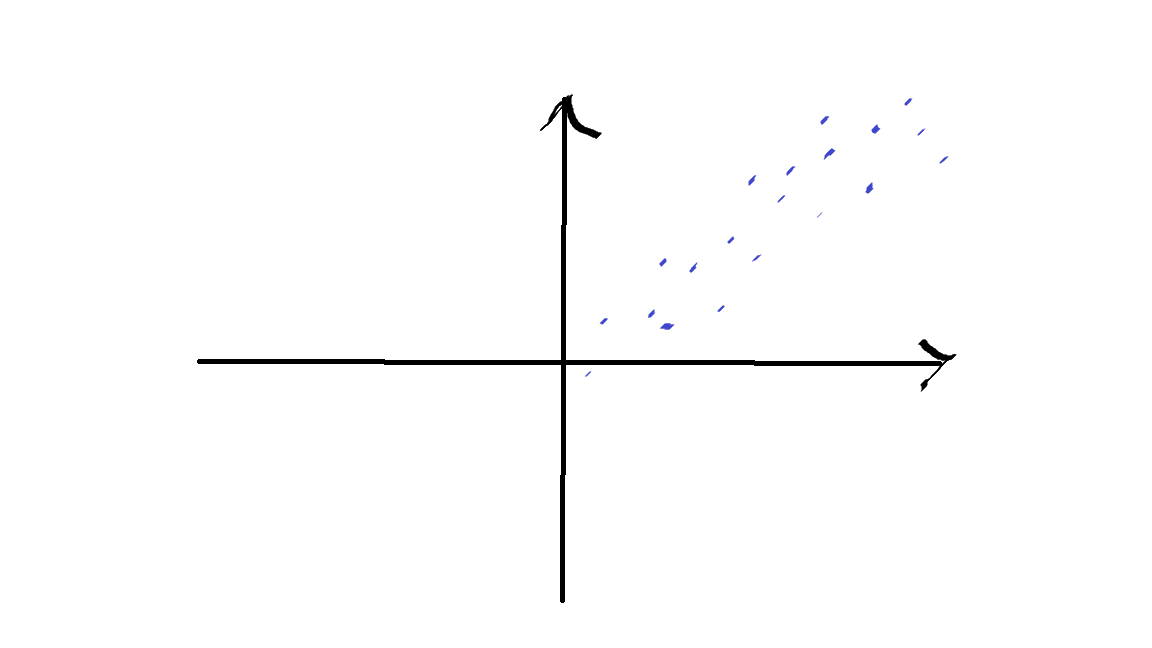
\includegraphics[scale =0.5]{C_and_A.png}

\easysubproblem{Give an example of two variables that are not correlated but are associated by drawing a plot.}\spc{4}
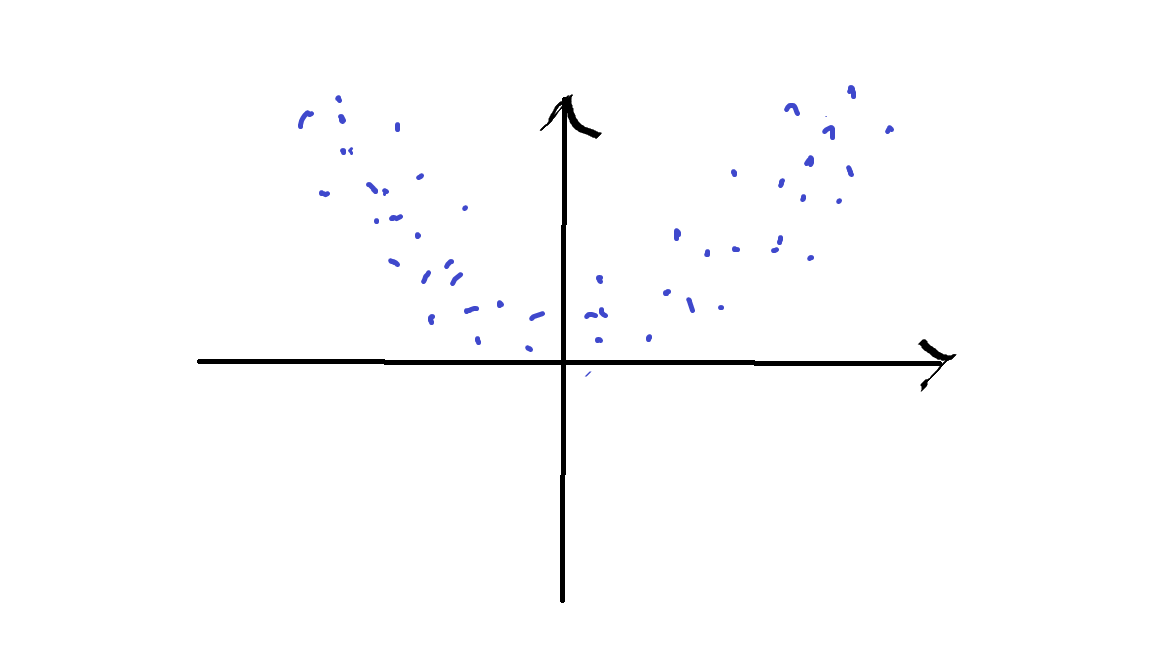
\includegraphics[scale =0.5]{A_and_not_C.png}

\easysubproblem{Give an example of two variables that are not correlated nor associated by drawing a plot.}\spc{4}
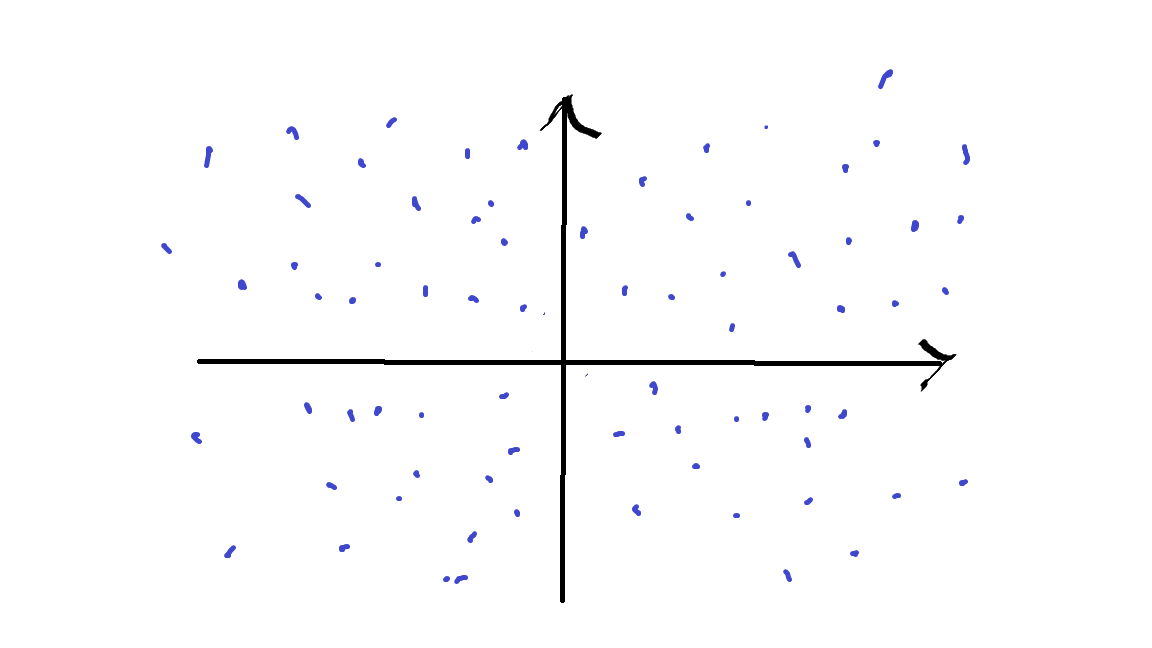
\includegraphics[scale =0.5]{not_A_and_not_C.png}

\easysubproblem{Can two variables be correlated but not associated? Explain.}\spc{4}

No. Correlation is a subset of association which refers to a linear relationship between variables. Variables that aren't associated, have no relationship. 


\end{enumerate}

\problem{These are questions about multivariate linear model fitting using the least squares algorithm.}

\begin{enumerate}

\hardsubproblem{Derive $\partialop{\c}{\c^\top A \c}$ where $\c \in \reals^n$ and $A \in \reals^{n \times n}$ but \textit{not} symmetric. Get as far as you can.}\spc{8}

$\c^\top A \c = \begin{bmatrix}
c_1 & c_2 & \dots & c_n 
\end{bmatrix}
\cdot
\begin{bmatrix}
a_{11} & a_{12} & \dots & a_{1n}\\
\hdotsfor{4}\\
a_{n1} & a_{n2} & \dots & a_{nn}
\end{bmatrix}
\cdot
\begin{bmatrix}
c_1\\
c_2\\
\dots \\
c_n
\end{bmatrix}$ \newline 
$= \begin{bmatrix}
c_1 & c_2 & \dots & c_n 
\end{bmatrix} 
\cdot 
\begin{bmatrix}
c_1 a_{11} + c_2 a_{12} + \ \dots \ +c_n  a_{1n}\\
c_1 a_{21} + c_2 a_{22} + \ \dots \  +c_n  a_{2n}\\
\hdotsfor{1}\\
c_1 a_{n1} + c_2 a_{n2} + \ \dots \  + c_n a_{nn}
\end{bmatrix}$ \newline 

$ = c_1 \big( c_1 a_{11} + c_2 a_{12} + \ \dots \ +c_n  a_{1n} \big) + c_2 \big( c_1 a_{21} + c_2 a_{22} + \ \dots \  +c_n  a_{2n} \big) + \ \dots \ + c_n \big( c_1 a_{21} + c_2 a_{22} + \ \dots \  +c_n  a_{2n} \big) $ \newline

$= \sum_{i=1}^n c_i \bigg( \sum_{j=1}^n  c_j a_{ij} \bigg)$ \newline 

$ \partialop{\c_i}{\c^\top A \c} = \partialop{\c_i}{\sum_{i, j=1}^n c_i c_j a_{ij}} $ \newline 

$ \hspace*{2.3cm}  =  \sum_{j=1}^n c_j a_{ij} + c_j a_{ji}$

\easysubproblem{Given matrix $X \in \reals^{n \times (p+1)}$, full rank and first column consisting of the $\onevec_n$ vector, rederive the least squares solution $\b$ (the vector of coefficients in the linear model shipped in the prediction function $g$). No need to rederive the facts about vector derivatives.}\spc{10}

$SSE = \sum \big(\vec{y_i} - \vec{\yhat_i} \big)^2 = \big( \vec{y} - \vec{\yhat} \big)^T \big( \vec{y} - \vec{\yhat} \big) = \big( \vec{y}^T - \vec{\yhat}^T \big) \big( \vec{y} - \vec{\yhat} \big)$ \newline 

$ \hspace*{9mm} = \vec{y}^T \vec{y} - \vec{y}^T\vec{\yhat} -  \vec{\yhat}^T \vec{y} + \vec{\yhat}^T \vec{\yhat}  $ \newline 

$ \hspace*{9mm} = \vec{y}^T \vec{y} - 2\vec{\yhat}^T\vec{y} + \vec{\yhat}^T \vec{\yhat}$ \newline 

$ \hspace*{9mm} = \vec{y}^T \vec{y} - 2\big( X\vec{b}\big)^T\vec{y} + \big(X\vec{b} \big)^T \big( X\vec{b} \big)$ \newline 

$ \hspace*{9mm} = \vec{y}^T \vec{y} - 2 \vec{b}^T X^T\vec{y} + \vec{b}^T X^T X \vec{b} $ \newline 

$ \frac{\partial}{\partial \vec{b}} \big[ \vec{y}^T \vec{y} - 2 \vec{b}^T X^T\vec{y} + \vec{b}^T X^T X \vec{b} \big] =  - 2 X^T\vec{y} +2 X^T X \vec{b} = 0 $ \newline 

$\big( X^T X \big)^{-1} \big( X^T X\big) \vec{b} = \big( X^T X)^{-1} X^T \vec{y}$ \newline 

$\vec{b} = \big(X^T X\big)^{-1} X^T \vec{y}$


\intermediatesubproblem{Consider the case where $p = 1$. Show that the solution for $\b$ you just derived is the same solution that we proved for simple regression in Lecture 8. That is, the first element of $\b$ is the same as $b_0 = \ybar - r \frac{s_y}{s_x}\xbar$ and the second element of $\b$ is $b_1 = r \frac{s_y}{s_x}$.} \spc{10}

$\vec{b} = \big(X^T X\big)^{-1} X^T \vec{y}$ \newline 

$ X \in \mathbb{R}^{n \times 2} = \begin{bmatrix}
    1       & x_{1} \\
    1      & x_{2}  \\
    \hdotsfor{2} \\
    1       & x_{n} 
\end{bmatrix}$ \newline 

$ X^T X =     \begin{bmatrix}
    1   & 1 & \dots & 1 \\
    x_1 & x_2 & \dots & x_n
    \end{bmatrix} 
    \cdot 
\begin{bmatrix}
    1       & x_{1} \\
    1      & x_{2}  \\
    \hdotsfor{2} \\
    1       & x_{n} 
    \end{bmatrix}
    = 
        \begin{bmatrix}
    n  & \sum x_i  \\
    \sum x_i & \sum x_i^2
    \end{bmatrix}$ \newline 
$ \sum x_i = n\xbar$ \newline 

$\big( X^T X\big)^{-1} = \frac{1}{n\sum x_i^2 -n^2 \xbar^2} \begin{bmatrix}
\sum x_i^2 & -n\xbar \\
-n\xbar & n 
\end{bmatrix}$ \newline 

$ \big( X^T X\big)^{-1} \big( X^T \vec{y} \big) =  \frac{1}{n\sum x_i^2 -n^2 \xbar^2} \begin{bmatrix}
\sum x_i^2 & -n\xbar \\
-n\xbar & n 
\end{bmatrix} 
\cdot 
\begin{bmatrix}
    1   & 1 & \dots & 1 \\
    x_1 & x_2 & \dots & x_n
    \end{bmatrix} 
\cdot
\begin{bmatrix}
 y_1 \\
 y_2 \\
 \dots \\
 y_n
 \end{bmatrix}$ \newline 
 
 $ \hspace*{3.1cm} = \frac{1}{n\sum x_i^2 -n^2 \xbar^2} \begin{bmatrix}
\sum x_i^2 & -n\xbar \\
-n\xbar & n 
\end{bmatrix}
\cdot 
\begin{bmatrix}
n\ybar \\
\sum y_i x_i
\end{bmatrix}$ \newline 

$ \hspace*{3.1cm} = \frac{1}{n\sum x_i^2 -n^2 \xbar^2} \begin{bmatrix}
n \ybar \sum x_i^2 -n \bar \sum y_i x_i \\
-n^2 \xbar \ybar +n \sum y_i x_i 
\end{bmatrix}$ \newline 

$b_0 = \frac{\ybar \big( \sum x_i ^2 -n \xbar^2 \big) - \xbar \big( \sum y_i x_i -n \xbar \ybar \big)}{\sum x_i^2 -n \xbar^2}$ \newline 

$b_1 = \frac{\sum y_i x_i - n \xbar \ybar}{\sum x_i^2 -n \xbar^2}$ \newline 


    
    

\easysubproblem{If $X$ is rank deficient, how can you solve for $\b$? Explain in English.} \spc{2}

Eliminate linearly dependent feature columns in the data matrix, until $X$ is full rank. 

\hardsubproblem{Prove $\rank{X} =\rank{X^\top X}$.}\spc{6}

$\rank{x}$ = Dim of whole space - $N(X)$ \newline 

Prove that $N(A) = N(A^TA)$: \newline 
$ N(A) \subset N(A^T A)$ \newline 
$ x \in N(A)$ \newline 
$Ax = 0$ \newline 
$A^T A x = A^T 0 = 0 \hspace*{1.5cm} \Rightarrow \hspace*{1.5cm} x\in N(A^TA)$ \newline 
so $ N(A) \subset N(A^T A)$ \newline 
$N(A^TA) \subset N(A)$ \newline 
$x \in N(A^T A)$ \newline 
$A^T Ax = 0$ \newline 
$x^T A^T a x = x^T 0 = 0$ \newline 
$(Ax)^T (Ax) =0$ \newline 
$ \vert \vert Ax \vert \vert^2 = 0$ \newline 
$Ax = 0$ \newline 
so $N(A^T A) \subset N(A)$ \newline 

Therefore, $N(X) = N(X^T X)$ and $\rank{X} = \rank{X^T X}$




\hardsubproblem{Given matrix $X \in \reals^{n \times (p+1)}$, full rank and first column consisting of the $\onevec_n$ vector, now consider cost multiples (\qu{weights}) $c_1, c_2, \ldots, c_n$ for each mistake $e_i$. As an example, previously the mistake for the 17th observation was $e_{17} := y_{17} - \hat{y}_{17}$ but now it would be $e_{17} := c_{17} (y_{17} - \hat{y}_{17})$.  Derive the weighted least squares solution $\b$. No need to rederive the facts about vector derivatives. Hints: (1) show that SSE is a quadratic form with the matrix $C$ in the middle (2) Split this matrix up into two pieces i.e. $C = C^{\half} C^{\half}$, distribute and then foil (3) note that a scalar value equals its own transpose and (4) use the vector derivative formulas.}\spc{20}

$SSE = \big( \y - X \vec{b} )^\top C \big( \y - X\vec{b} \big)$  \\
$ \hspace*{1cm} = \big( \y^\top C\y - \y^\top CX\vec{b} - \vec{b}^\top X^\top C \y +\vec{b} ^\top X^\top C X b \big)$ \\

$\frac{\partial SSE}{\partial \vec{b}} \ = \ -2X^\top C\y +2X^\top C X \vec{b} \ = \ 0$ \\

$ \vec{b} = \big(X^\top C X )^{-1} X^\top C \y$




\hardsubproblem{If $p=1$, prove $r^2 = R^2$ i.e. the linear correlation is the same as proportion of sample variance explained in a least squares linear model.}\spc{6}

$b_1 = \frac{\sum (x_i - \xbar)(y_i - \ybar)}{\sum (x_i - \xbar)^2}$ \\
$b_0 = \ybar - b_1 \xbar$ \\
$\yhat_i = b_0 +b_1 x_i \ = \ \ybar - \bigg[ \frac{\sum (x_i - \xbar)(y_i - \ybar)}{\sum (x_i - \xbar)^2} \bigg] \xbar \ + \ \bigg[ \frac{\sum (x_i - \xbar)(y_i - \ybar)}{\sum (x_i - \xbar)^2} \bigg]x_i $ \\

$$R^2 = \frac{SSR}{SST}$$ 
$$ \ \ = \frac{\sum (\yhat_i - \ybar)^2}{\sum (y_i -\ybar)^2}$$
$$ \ \ = \frac{\sum \bigg( \ybar - \bigg[ \frac{\sum (x_i - \xbar)(y_i - \ybar)}{\sum (x_i - \xbar)^2} \bigg] \xbar \ + \ \bigg[ \frac{\sum (x_i - \xbar)(y_i - \ybar)}{\sum (x_i - \xbar)^2} \bigg]x_i -\ybar \bigg)^2}{\sum \big(y_i -\ybar \big)^2}$$
$$ \ \ = \frac{\sum \bigg(  \frac{\sum (x_i - \xbar)(y_i - \ybar)}{\sum (x_i - \xbar)^2}  \bigg)^2 \big(x_i - \xbar \big)^2}{\sum \big(y_i -\ybar \big)^2}$$
$$ \ \ = \frac{\big[ \sum \big(x_i - \xbar \big) \big( y_i -\ybar \big) \big]^2}{\sum \big( x_i -\xbar \big)^2 \sum \big( y_i -\ybar \big)^2}$$
$$ \ \ = \frac{\big[ Cov(x, y) \big]^2}{s_x ^2 s_y^2}$$
$$ \ \ = r^2$$

\intermediatesubproblem{Prove that the point $<1,\xbar_1, \xbar_2, \ldots, \xbar_p, \bar{y}>$ is a point on the least squares linear solution.}\spc{13}

Show that $\begin{bmatrix}
1 & \xbar_1 & \xbar_2 & \dots & \xbar_{p+1}
\end{bmatrix}
\vec{b} = \ybar$ \\
%$\yhat = b_0 + b_1 x_1 \ + \ b_2 x_2 \ + \ \dots \ + \ b_{p+1} x_{p+1}$ \\
$$\yhat^{*} = b_0 + b_1 \xbar_1 \ + \ b_2 \xbar_2 \ + \ \dots \ + \ b_{p+1} \xbar_{p+1}$$
$$ \yhat^{*} = \frac{1}{n} \sum b_0 + \frac{1}{n} \sum b_1 x_{i1} \ + \ \frac{1}{n} \sum b_2 x_{i2} \ + \ \dots \ + \ \frac{1}{n} \sum b_{p+1} x_{i p+1}$$
Since $\yhat_i = b_0 + b_1 x_{i1} \ + \ b_2 x_{i2} \ + \ \dots \ + \ b_{i p+1} x_{ ip+1}$ \\
$$\yhat^{*} = \frac{1}{n} \sum \yhat_i$$
As proven on previous homework, $\frac{1}{n} \sum \big( \y_i - \yhat_i \big) \ = \ \frac{1}{n} \sum e_i \ = \ 0$ \\
Therefore, $\frac{1}{n} \sum \yhat_i  =  \frac{1}{n} \sum \y_i = \ybar$\\
Thus, $$\yhat^{*} = \ybar = b_0 + b_1 \xbar_1 \ + \ b_2 \xbar_2 \ + \ \dots \ + \ b_{p+1} \xbar_{p+1}$$


\end{enumerate}

\problem{These are questions related to the concept of orthogonal projection, QR decomposition and its relationship with least squares linear modeling.}

\begin{enumerate}

\easysubproblem{Consider least squares linear regression using a design matrix $X$ with rank $p + 1$. What are the degrees of freedom in the resulting model? What does this mean?}\spc{3}

There are p+1 degrees of freedom. This means that the resulting model: $ \yhat = w_0 + w_1 x_1 + \dots +w_p x_p$  has p+1 weight parameters that can be adjusted. 

\intermediatesubproblem{If you are orthogonally projecting the vector $\y$ onto the column space of $X$ which is of rank $p + 1$, derive the formula for $\proj{\colsp{X}}{\y}$. Is this the same as the least squares solution?}\spc{6}

$\proj{\colsp{X}}{\y} = X \vec{w}$ \newline 
$X^T \big( \y -X\vec{w} \big) = 0$   Because of orthogonality \newline 
$X^T \y - X^TX \vec{w} = 0$ \newline 
$X^T \y = X^TX \vec{w}$ \newline 
$ \vec{w} = \big( X^T X \big)^{-1}X^T \y$ \newline 
$\proj{\colsp{X}}{\y} = X \vec{w} = X \big( X^T X \big)^{-1}X^T \y = H\y$ \newline 

Yes. This is the same as the least squares solution. 



\hardsubproblem{We saw that the perceptron is an \textit{iterative algorithm}. This means that it goes through multiple iterations in order to converge to a closer and closer $\w$. Why not do the same with linear least squares regression? Consider the following. Regress $\y$ using $\X$ to get $\yhat$. This generates residuals $\e$ (the leftover piece of $\y$ that wasn't explained by the regression's fit, $\yhat$). Now try again! Regress $\e$ using $\X$ and then get new residuals $\e_{new}$. Would $\e_{new}$ be closer to $\zerovec_n$ than the first $\e$? That is, wouldn't this yield a better model on iteration \#2? Yes/no and explain.}\spc{10}

No. The projection onto $\colsp{X}$ gives the minimum square error on the first iteration. Going through that process again would yeild the same result because of the idempotency of the projection matrix. \\
$ H = X \big( X^T X \big)^{-1}X^T$ and $ H \cdot H = H$


\intermediatesubproblem{Prove that $Q^\top = Q^{-1}$ where $Q$ is an orthonormal matrix such that $\colsp{Q} = \colsp{X}$ and $Q$ and $X$ are both matrices $\in \reals^{n \times (p+1)}$. Hint: this is purely a linear algebra exercise.}\spc{10}

Prove: $Q^\top Q =I$ \\

$$
\begin{bmatrix}
\leftarrow & q_{\cdot 1} & \rightarrow\\
\leftarrow & q_{\cdot 2} & \rightarrow \\
 & \dots &  \\
 \leftarrow & q_{\cdot n} & \rightarrow\\
\end{bmatrix}
\cdot 
\begin{bmatrix}
\uparrow & \uparrow &  & \uparrow \\
q_{\cdot 1} & q_{\cdot 2} & \dots & q_{\cdot n}\\
\downarrow & \downarrow & & \downarrow
\end{bmatrix}
=
\begin{bmatrix}
q_{\cdot 1}^\top q_{\cdot 1} & q_{\cdot 1}^\top q_{\cdot 2} & \dots & q_{\cdot 1}^\top q_{\cdot n} \\
q_{\cdot 2}^\top q_{\cdot 1} & q_{\cdot 2}^\top q_{\cdot 2} & \dots & q_{\cdot 2}^\top q_{\cdot n} \\
\dots & \dots & \dots & \dots  \\
q_{\cdot n}^\top q_{\cdot 1} & q_{\cdot n}^\top q_{\cdot 2} & \dots & q_{\cdot n}^\top q_{\cdot n} \\
\end{bmatrix}$$
$q_{\cdot i}^\top q_{\cdot i} = \vert \vert q_{\cdot i} \vert \vert ^2$,   and $q_{\cdot i}^\top q_{\cdot j} = 0$ when $i \neq j$ because of orthonormality of $Q$. \\
$$ Q^\top Q= \begin{bmatrix}
1 & 0 & \dots & 0 \\
0 & 1 & \dots & 0 \\
\dots & \dots & \dots & \dots  \\
0 & 0 & \dots & 1 \\
\end{bmatrix}
=I$$


\intermediatesubproblem{Prove that the least squares projection $H = \XXtXinvXt$ is the same as $QQ^\top$.}\spc{10}

In previous part I proved: $Q^\top Q = I$ \newline 

Show that $QQ^T = X \big( X^T X \big)^{-1} X^T$ \newline 
$\big( QR \big) \Big( \big(QR \big)^T QR \Big)^{-1} \big( QR\big)^T$ \newline 
$ = QR \big( R^TQ^T Q Q)^{-1}R^TQ^T$ \newline 
$ = QR \big(R^T I R \big)^{-1} R^T Q^T$ \newline 
$ = QR \big(R^T R \big)^{-1} R^T Q^T$ \newline 
$ = QR R^{-1} (R^T)^{-1} R^T Q^T$ \newline 
$ = Q I IQ^T$ \newline 
$ = QQ^T$ 

\intermediatesubproblem{Prove that an orthogonal projection onto the $\colsp{Q}$ is the same as the sum of the projections onto each column of $Q$.}\spc{10}
 
Projection onto each column of $Q$:\\

$\proj{q_{\cdot i}}{\vec{a}} = \frac{q_{\cdot i} q_{\cdot i}^\top}{\vert \vert q_{\cdot i} \vert \vert ^2} \vec{a} $\\

Since Q is orthonormal, $\vert \vert q_{\cdot i} \vert \vert ^2 =1$, and $\proj{q_{\cdot i}}{\vec{a}} = q_{\cdot i} q_{\cdot i}^\top \vec{a}$ \\

$$\sum_{i= 1}^{p+1} \proj{q_{\cdot i}}{\vec{a}} = \sum_{i= 1}^{p+1} q_{\cdot i} q_{\cdot i}^\top \vec{a} \ = \ QQ^\top \vec{a}$$
Since all the columns in $Q$ are orthogonal to each other. 




\hardsubproblem{Trouble in paradise. Prove that the SSE of a multivariate linear least squares model always decreases (equivalently, $R^2$ always increases) upon the addition of a new independent predictor. Keep in mind this holds true even if this new predictor has no information about the true causal inputs to the phenomenon $y$.}\spc{12}

As SSR increases $\Rightarrow$ SSE decreases. This is because SST = SSR + SSE, and SST is a measure of variance in $\y$; it doesn't depend on the $x$'s or $g$. \\
Now, add a random $x_{p+2}$ column to $\mathcal{X}$. $\rank{X}$ = p+2. \\
$SSR_{new} =  \sum_{i=1}^{n} \big(\yhat_i - \ybar \big)^2 = \sum_{j =1}^{p+1} \vert \vert \proj{q\cdot  j}{\y} \vert \vert ^2 + \vert \vert \proj{q\cdot  p+2}{\y} \vert \vert^2 \ \geq SSR_{old}$ \\
Thus, $SSE_{new} \leq SSE_{old}$, and $R_{new}^2 \geq R_{old}^2$



\intermediatesubproblem{Why is this a bad thing? Explain in English.}\spc{3}

This means that any random, non orthogonal vector added to $\mathcal{X}$ would increase $R^2$. It makes it hard to determine whether or not the $x$'s in the model actually explain $\y$.  


\extracreditsubproblem{Prove that $\rank{H} =\tr{H}$.}\spc{-0.5}

\end{enumerate}


\end{document}
